\documentclass{article}
\usepackage{amsmath, amsthm, amssymb, amsfonts, bm}
\usepackage{graphicx}
\usepackage[T1]{fontenc}
\usepackage[utf8]{inputenc}
\usepackage[a4paper]{geometry}
\usepackage{fancyhdr}
\usepackage[algo2e]{algorithm2e}
\fontfamily{cmr}

\title{DD2424 - Assignment 3}
\author{Oskar Stigland \\ stigland@kth.se}

\pagestyle{fancy}
\fancyhf{}
\rhead{stigland@kth.se}
\lhead{DD2424 - Deep Learning in Data Science}
\rfoot{Page \thepage}

\begin{document}
%\maketitle

	\begin{titlepage}
		\begin{center} 
			
			\rule{\linewidth}{0.5mm}\\[0.5 cm]
			{ \huge \bfseries DD2424 - Assignment 3}\\[0.3 cm] % Title of your document
			\rule{\linewidth}{0.5mm}\\[1 cm]
					
			\small\vfill
			\begin{center}
			\centering
			{\large \bfseries \textsc{Summary}}\\
			\vspace{1cm}
			\begin{minipage}{10cm}
				
				I have implemented \texttt{batch normalization} and trained a $k$-layer network using cyclical learning rates. For the $3$-layer network with \texttt{batch normalization} and $50$ nodes in each hidden layer, I have implemented a $\lambda$-search and then trained the top-performing parameter setting for $3$ cycles, for which I achieved a $53.60$\% accuracy on the test set. However, this was still lower than for the standard $\lambda = 0.005$, for which accuracy on the test set was $53.76$\% with \texttt{batch normalization}. For the $9$-layer network, the corresponding performance with and without \texttt{batch normalization} was received $50.83$\% and $46.35$\%, respectively. However, as is clarified in the report, I have not achieved a perfect match for the analytical and numerical gradient calculations. More on this below.\\\\
%
	The code for the assignment has been written in \texttt{python}. I have implemented the neural network as a class. For the hand-in, all of the code has been put toghether in a main file with all the functions and the class declared at the top. For the hand-in, I have also commented out the saving of generated figures and results in JSON files, as well as omitting some of the case-specific testing and gradient testing.
			\end{minipage}
			\end{center}
			\large\vfill
						

		\end{center}	
		
		\begin{minipage}{0.4\textwidth}
			\begin{flushleft} \large
				%\emph{Student:}\\
				Oskar \textsc{Stigland}\\
				DD2424\\
				Spring 2023
			\end{flushleft}
		\end{minipage}	

	\end{titlepage}

\newpage

\subsection*{Checking gradients}

	In order to validate the anaytic gradient computations, I compared the analytically computed gradients with numerically computed gradients on a subset of the weights of a large subset of the training data using $h = 10^{-5}$.  I got that
	$$\vert\vert \nabla_{\bm{w}} \bm{J}- \nabla_{\bm{w}} \bm{J}^{\text{numerical}} \vert\vert_{\infty} < 10^{-9}, \quad \forall\bm{w} \in \bm{W}_k$$
	where $\bm{W}_k$ is the full set of weights for the final layer, including also the weights in the bias vector. I also had that
	$$\vert\vert \nabla_{\bm{w}} \bm{J} - \nabla_{\bm{w}} \bm{J}^{\text{numerical}} \vert\vert_{\infty} < 10^{-9}, \quad \forall\bm{w} \in \bm{\gamma}_{k-1}, \bm{\beta}_{k-1}$$
	where $\bm{\gamma}_{k-1}, \bm{\beta}_{k-1}$ are the full set of weight in the scale, $\gamma_{k-1}$, and shift, $\beta_{k-1}$, for the next-to-last layer, i.e. $\ell = k-1$. However, for the remaining weights in the network the difference was on the order of $10^{-2}$. The issue seems to arise when the gradients are propagated through the batch normalization, i.e. refered to as the \texttt{batchNormBackPass}. I have turned my code inside out several times, but can not seem to find the issue. It might also be that there is an issue in the numerical gradient calculations. When training a $5$-layer network with $[50, 50, 20, 30]$ hidden nodes - as well as a $9$-layer network with the same specs as in the assignment description - on a small subset of the training data with $\vert D\vert = 100$ and $500$ epochs, not using any regularization, I get the following results:
	\begin{figure}[h!]
		\centering
		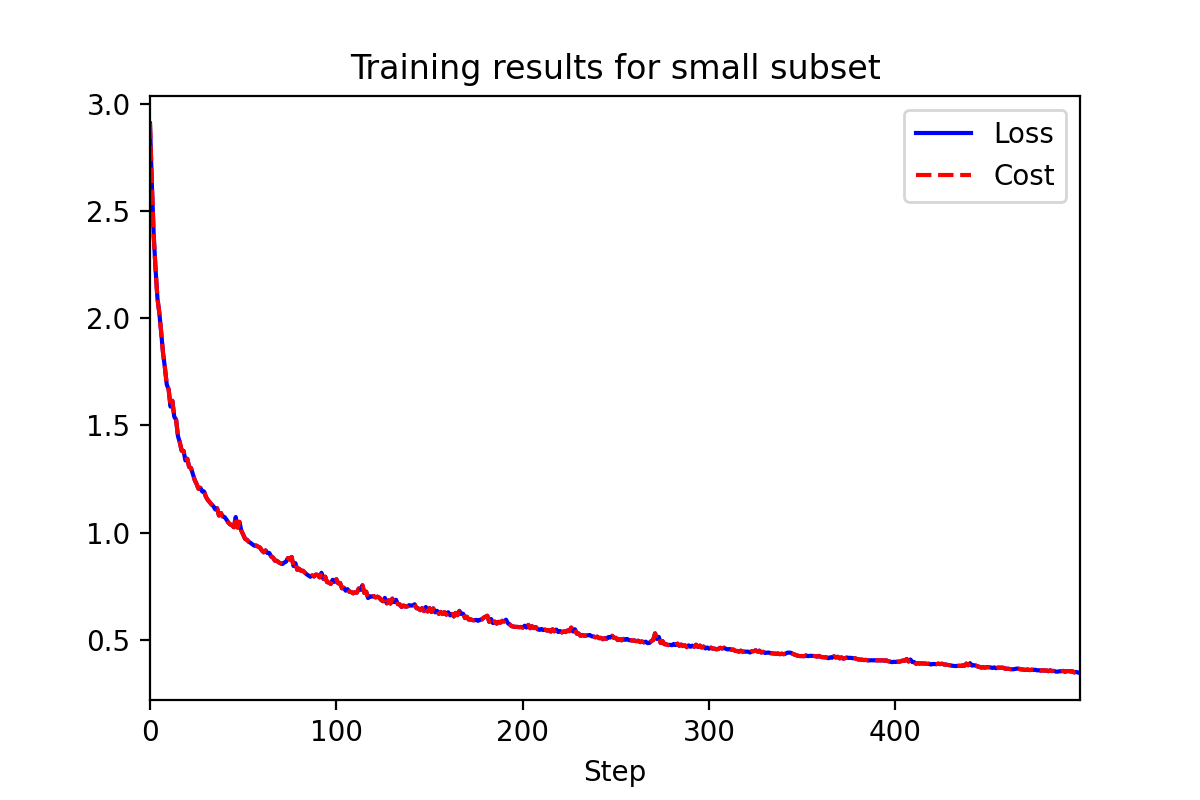
\includegraphics[width=7cm]{../plots/grad_test_5layer.png}
		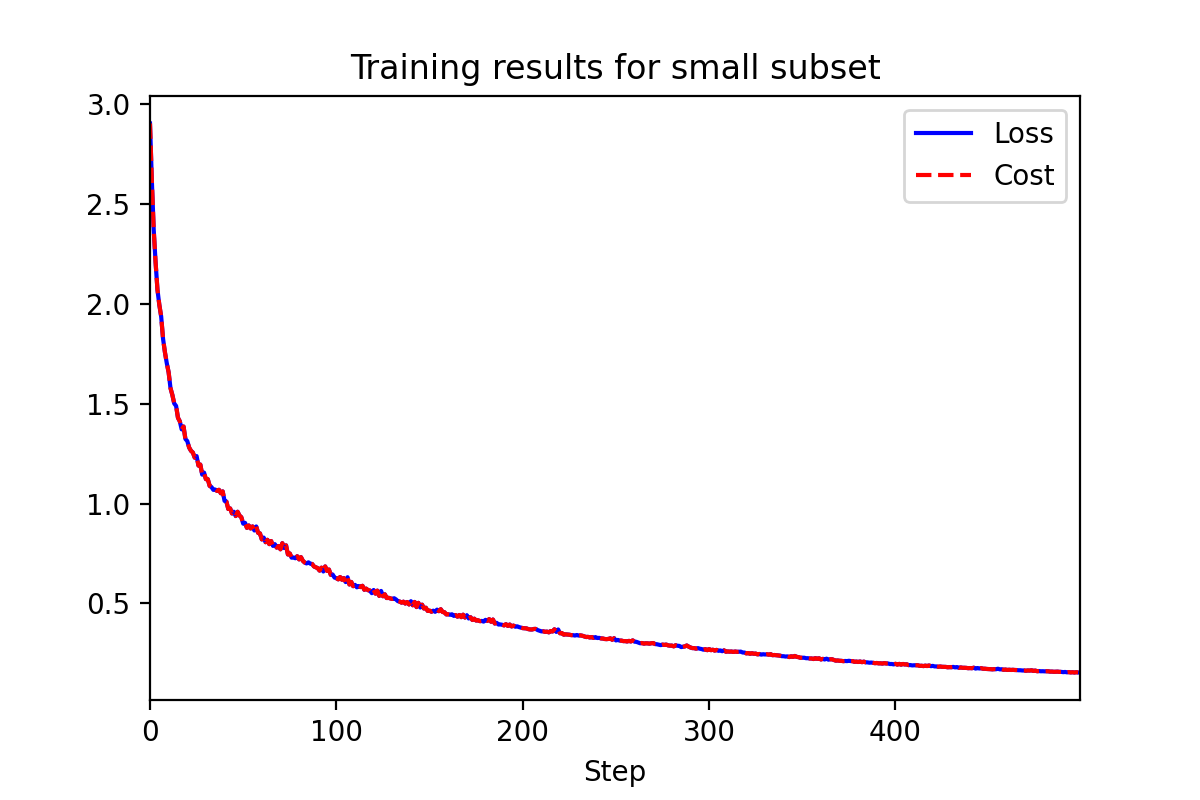
\includegraphics[width=7cm]{../plots/grad_test_9layer.png}
		\caption{Loss and cost for $5$-layer and $9$-layer network using \texttt{batch normalization} and $\eta=0.01$, $\lambda=0.0$, on $D\subset \bm{X}$, $\vert D\vert = 100$}
	\end{figure}\\
	Thus, I am confident the analytically computed gradients are \textbf{not} entirely bug free. Especially, the loss and cost gets increasingly unstable as the number of layers increase. However, despite the analytical gradients not being entirely bug-free, the multi-layer network seems to learn how to classify the CIFAR-10 fairly well, with testing accuracy above $50$\% during a normal training procedure with batch normalization and a cyclical learning rate. \\\\
%
For the $k$-layer network \textbf{without} \texttt{batch normalization}, the analytical gradients are seemingly bug free, with pairwise absolute difference between analytically and numerically computed gradients on the order of $10^{-10}$ for all weights.

\newpage
\subsection*{The effects of \texttt{batch normalization}}
\vspace{0.5cm}

\subsubsection*{Training a $3$-layer network}
	For the $3$-layer network, there is no discernable difference in terms of the performance of the networks with respect to the accuracy on the test dataset. In fact, omitting \texttt{batch normalization} seems to result in a more stable training procedure.
	\begin{figure}[h!]
		\centering
		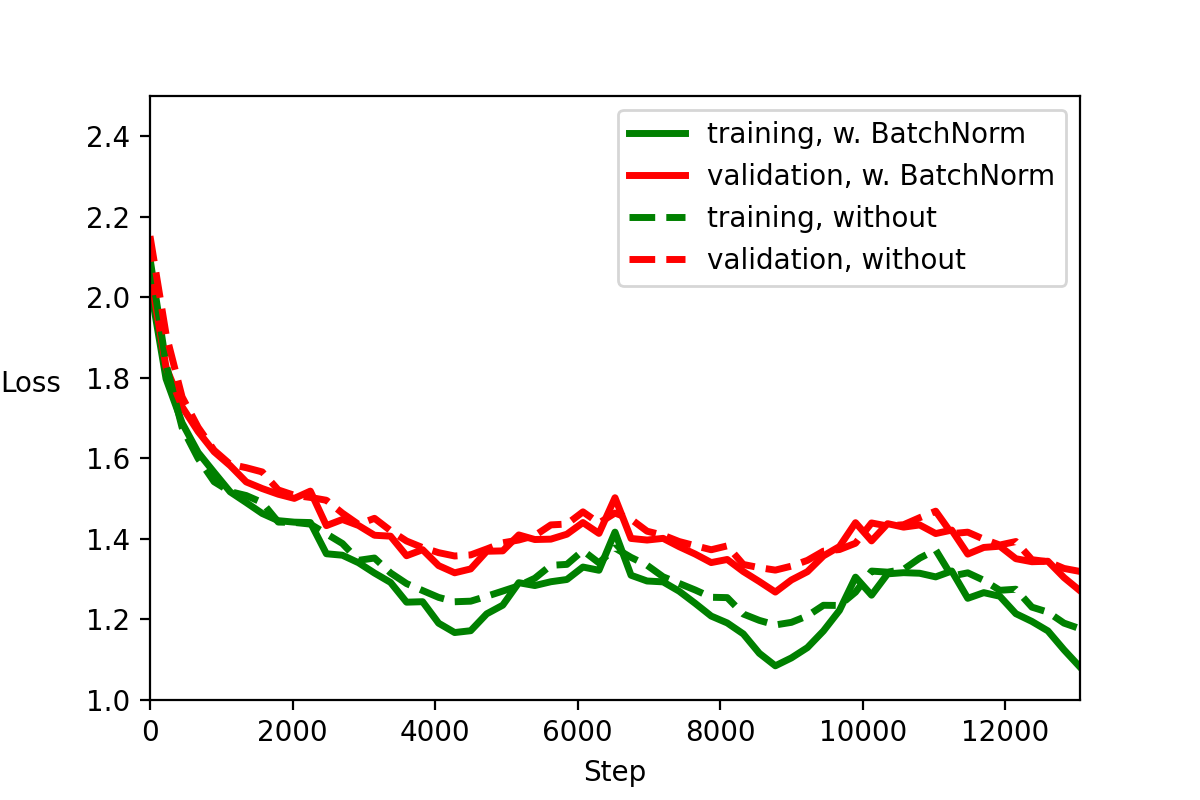
\includegraphics[width=7cm]{../plots/loss_comp_3layer.png}
		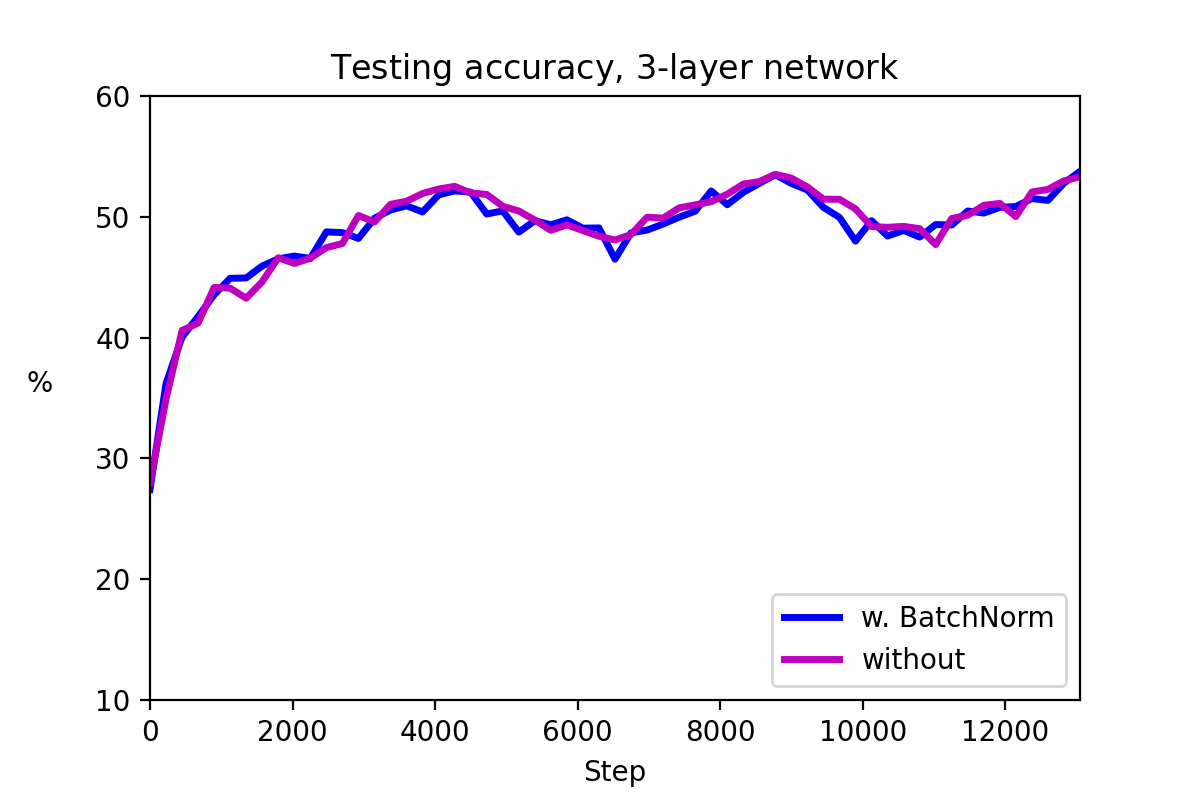
\includegraphics[width=7cm]{../plots/acc_comp_3layer.png}
		\caption{Loss and accuracy for $3$-layer network with and without \texttt{batch normalization}, using $\lambda=0.005$, and a cyclical learning rate with $\eta_{min} = 10^{-5}$ and $\eta_{max} = 10^{-1}$.}
	\end{figure}
\subsubsection*{Training a $9$-layer network}
	There is a clear difference when implementing and omitting \texttt{batch normalization}. In the former case, the network achieves an accuracy on the test dataset slightly above $50$\%, while the corresponding accuruacy in the latter case is on the order of $45$\%. There is also a clear difference in terms of the loss, where the network trained with \texttt{batch normalization} achieves a lower loss across the training process.
	\begin{figure}[h!]
		\centering
		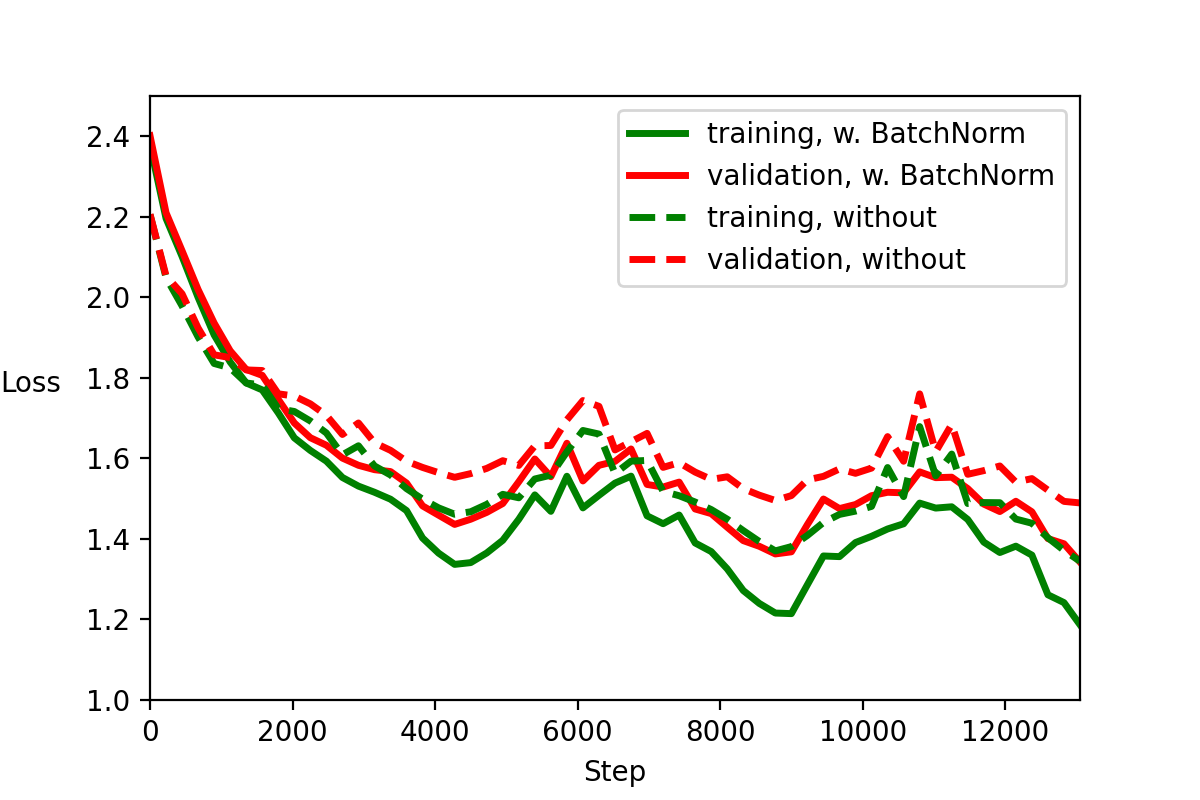
\includegraphics[width=7cm]{../plots/loss_comp_9layer.png}
		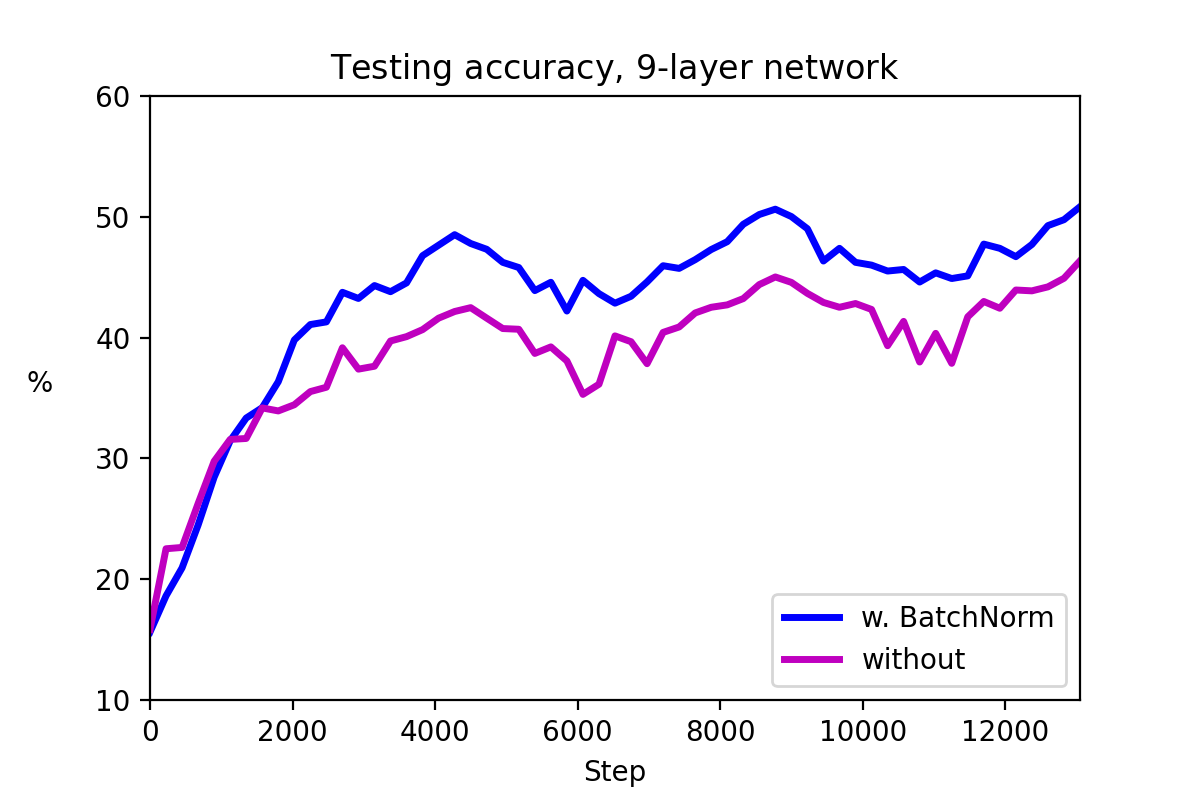
\includegraphics[width=7cm]{../plots/acc_comp_9layer.png}
		\caption{Loss and accuracy for $9$-layer network with and without \texttt{batch normalization}, using $\lambda=0.005$, and a cyclical learning rate with $\eta_{min} = 10^{-5}$ and $\eta_{max} = 10^{-1}$.}
	\end{figure}

\newpage
\subsection*{Conducting a $\lambda$-search}
	I conducted a search for an optimal $\lambda$ by computing $10^l$ where
	$$l = l_{min} + (l_{max} - l_{min}) \cdot u, \quad u\sim\text{Uniform}(0, 1)$$
	and $l_{min} = -4$ and $l_{max} = -2$, by sampling $u$ for a number of iterations and training for $2$ cycles per iteration. I achieved the best highest accuracy on the test dataset with $\lambda = 0.0093$. Then, I trained a network with $\lambda = 0.009$ for $3$ cycles and attained an accuracy of $53.60$\%. The loss, cost and accuracy are plotted below. In general, it seems that the multi-layer network with \texttt{batch normalization} benefits from a higher rate of regularization in comparison to the network in the previous assignment, where I found an optimal $\lambda$ to be more on the order of $\leq 0.0002$.

	\begin{figure}[h!]
		\centering
		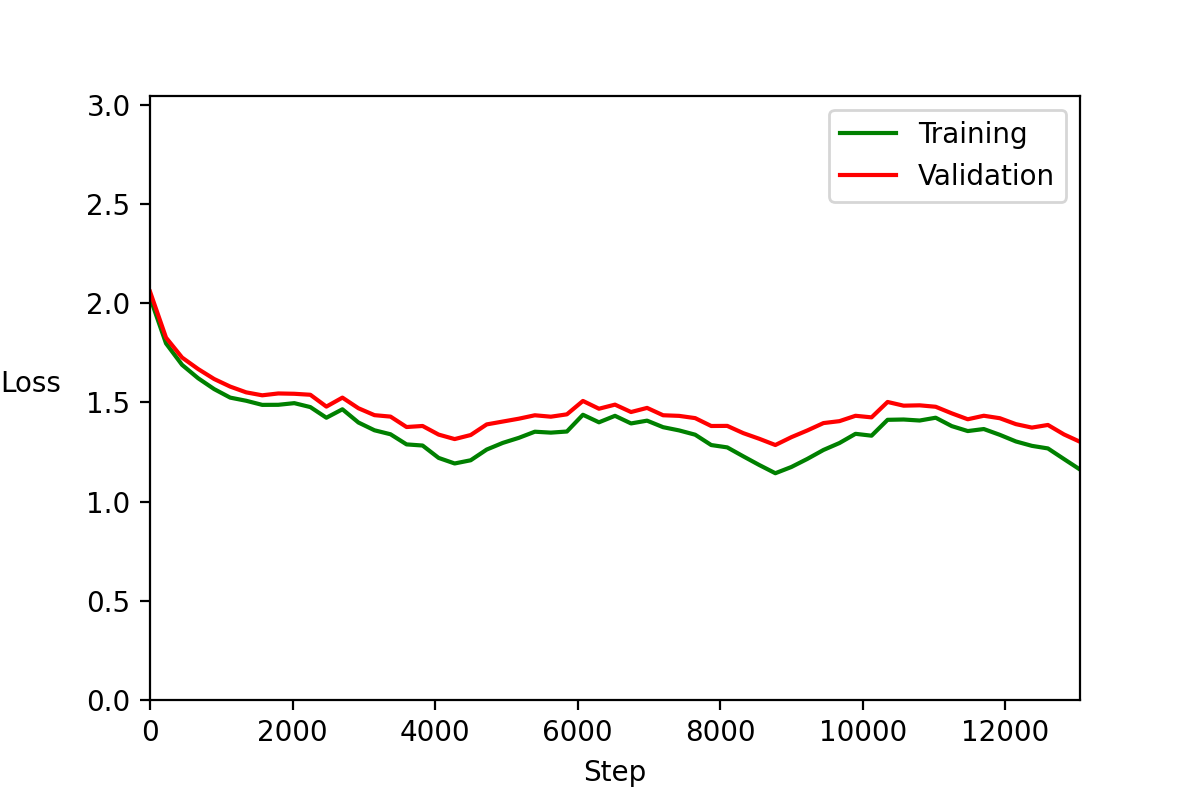
\includegraphics[width=7cm]{../plots/loss_lambdaOptimal.png}
		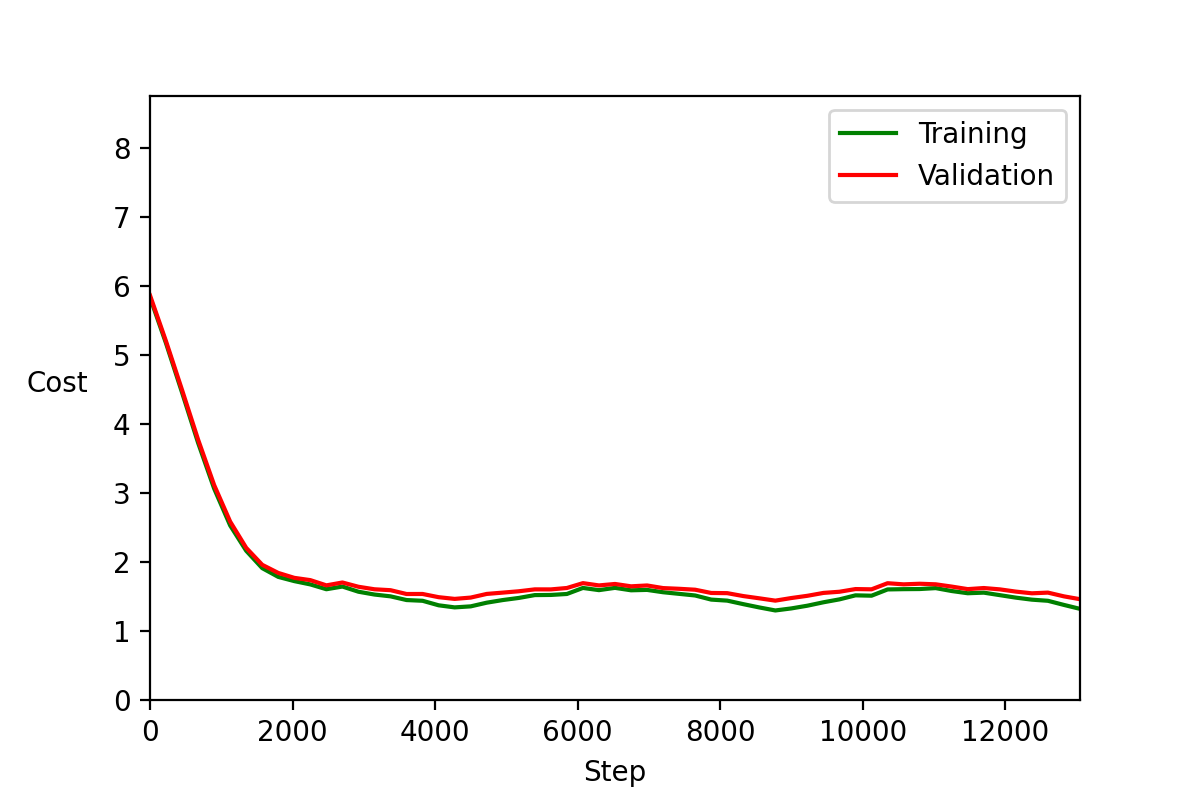
\includegraphics[width=7cm]{../plots/cost_lambdaOptimal.png}
		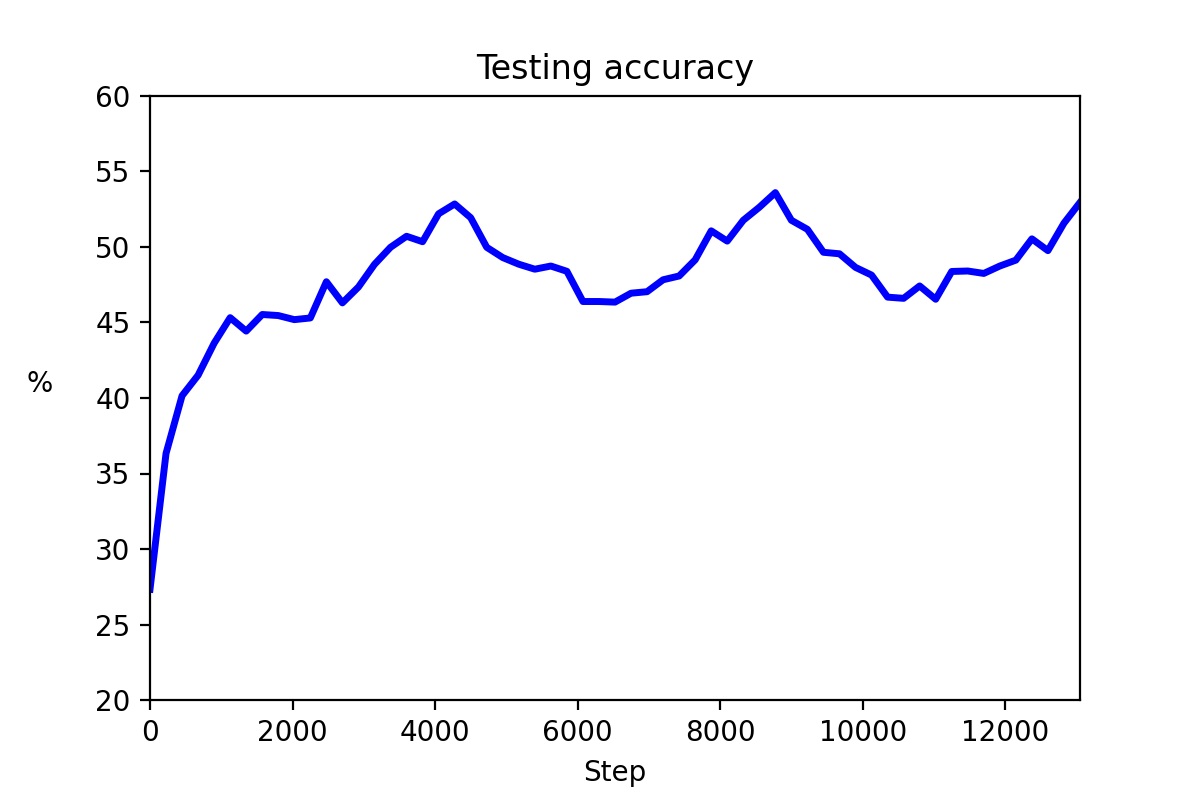
\includegraphics[width=8cm]{../plots/acc_lambdaOptimal.png}
		\caption{Loss , cost and testing accuracy for $3$-layer neural network with batch normalization and $m = 50$ nodes in each hidden layer, using $\lambda=0.009$, $\eta_{min}=10^{-5}$,  $\eta_{max}=10^{-1}$, and $ns = 2250$ for $3$ cycles.}
 	\end{figure}

\newpage
\subsection*{Sensitivity to initialization}
	When we decrease the variance in the random normal initialization of $\bm{W}$, we get an increasingly poor training performance in the case where \texttt{batch normalization} is omitted. In the third case, where $\bm{W}$ are initialized with $\mathcal{N}(0, 0.0001)$, there is in fact no learning whatsoever. On the other hand, in the case of implementing \texttt{batch normalization}, the loss during training and accuracy during testing seems to be pretty much equal across all three cases.
	\begin{figure}[h!]
		\centering
		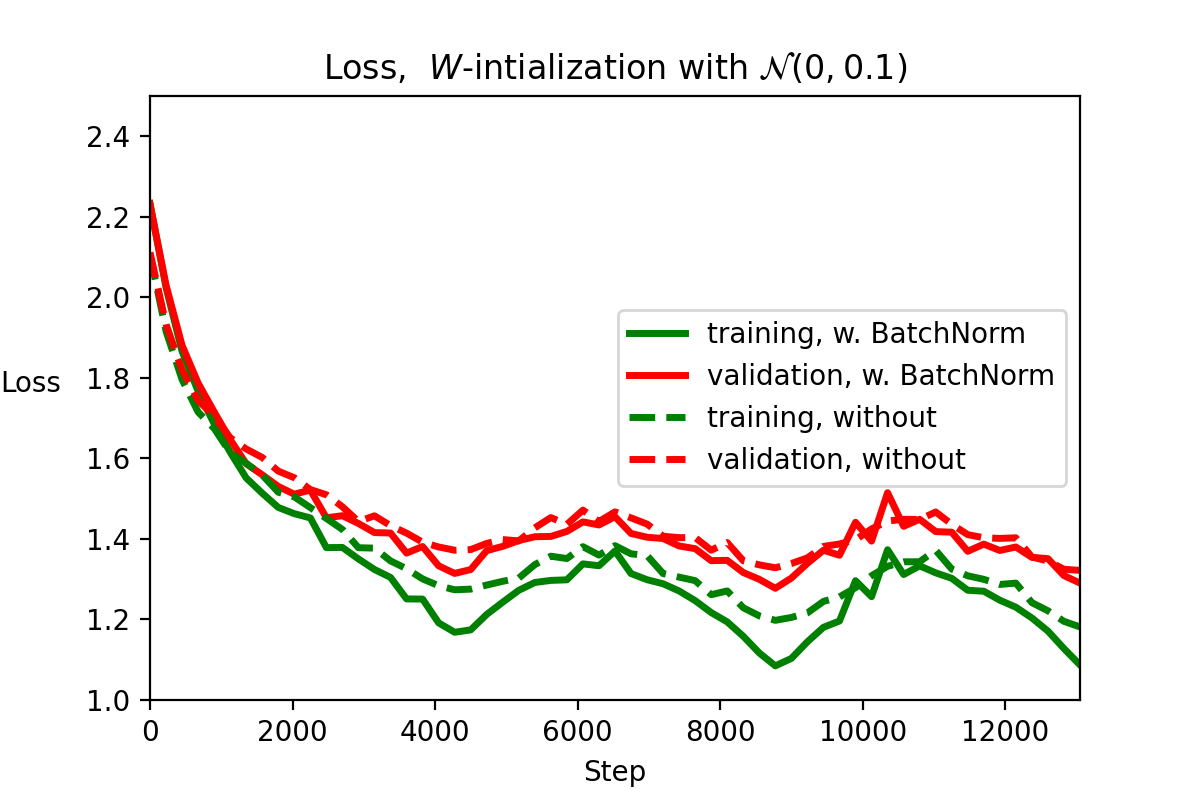
\includegraphics[width=7cm]{../plots/loss_comp_sigma1.png}
		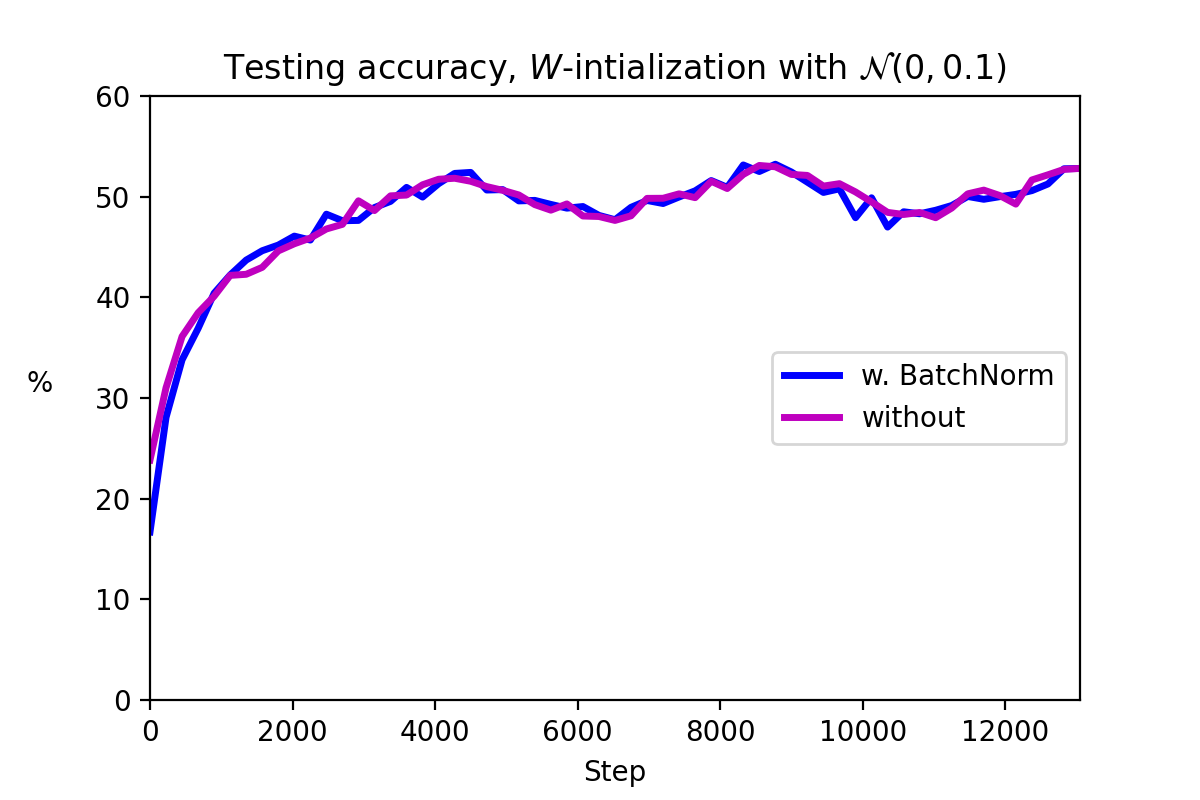
\includegraphics[width=7cm]{../plots/acc_comp_sigma1.png}
		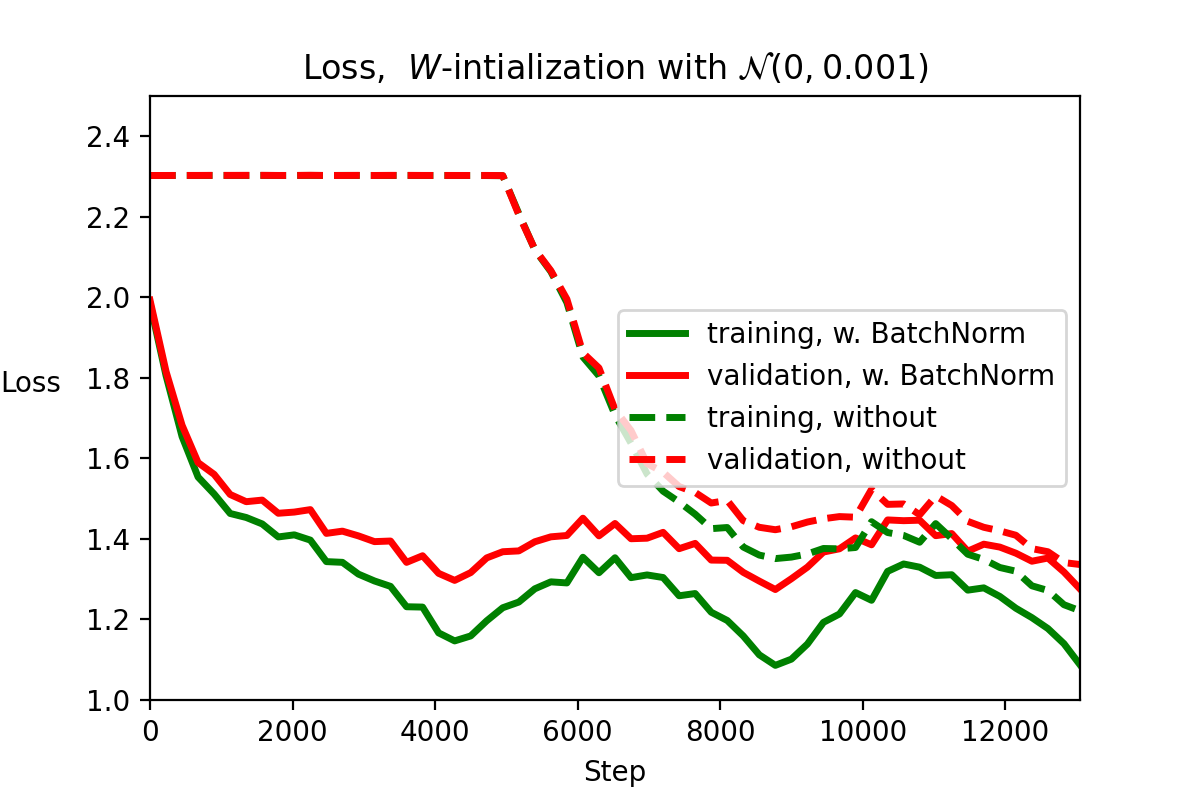
\includegraphics[width=7cm]{../plots/loss_comp_sigma2.png}
		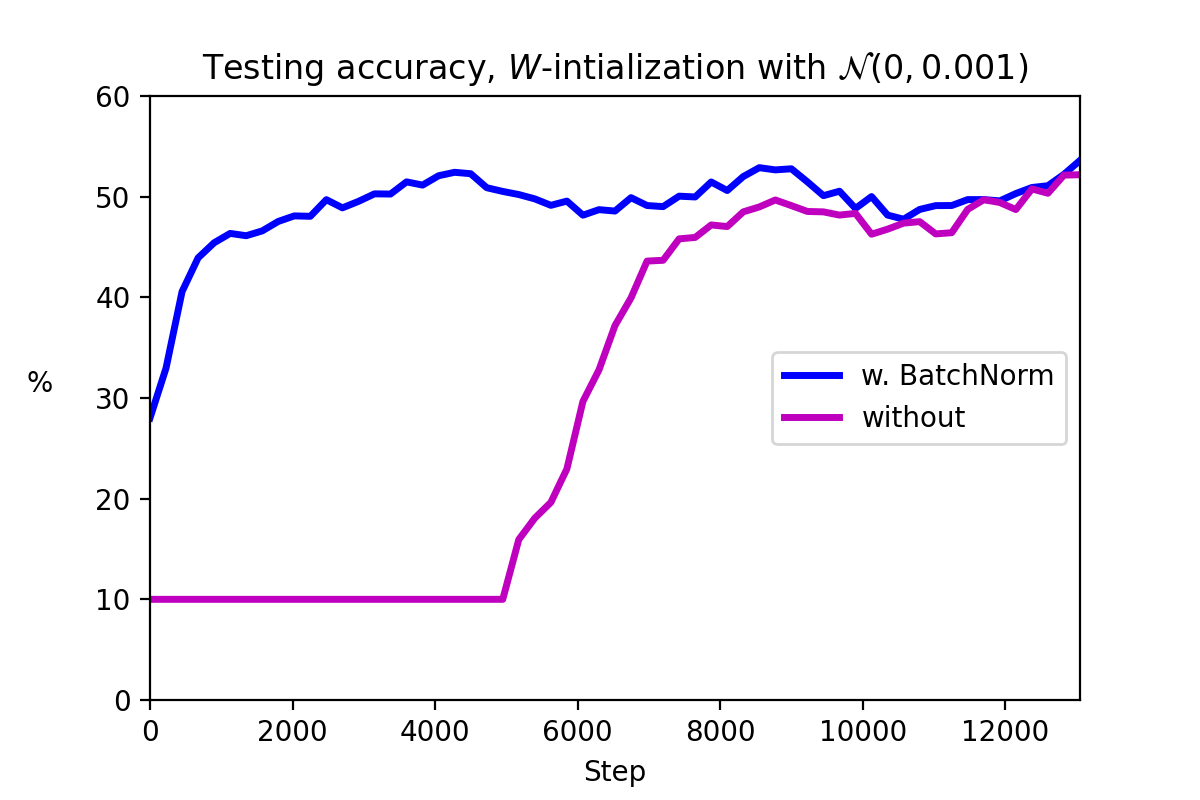
\includegraphics[width=7cm]{../plots/acc_comp_sigma2.png}
		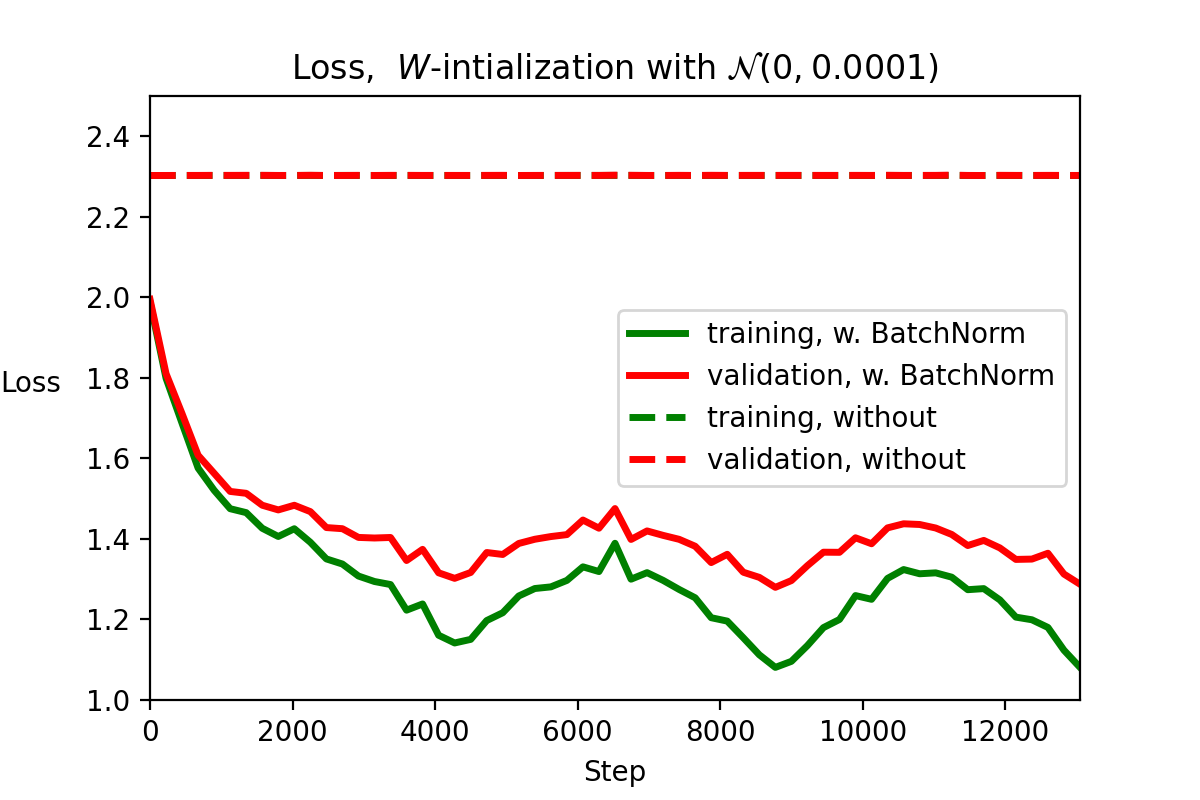
\includegraphics[width=7cm]{../plots/loss_comp_sigma3.png}
		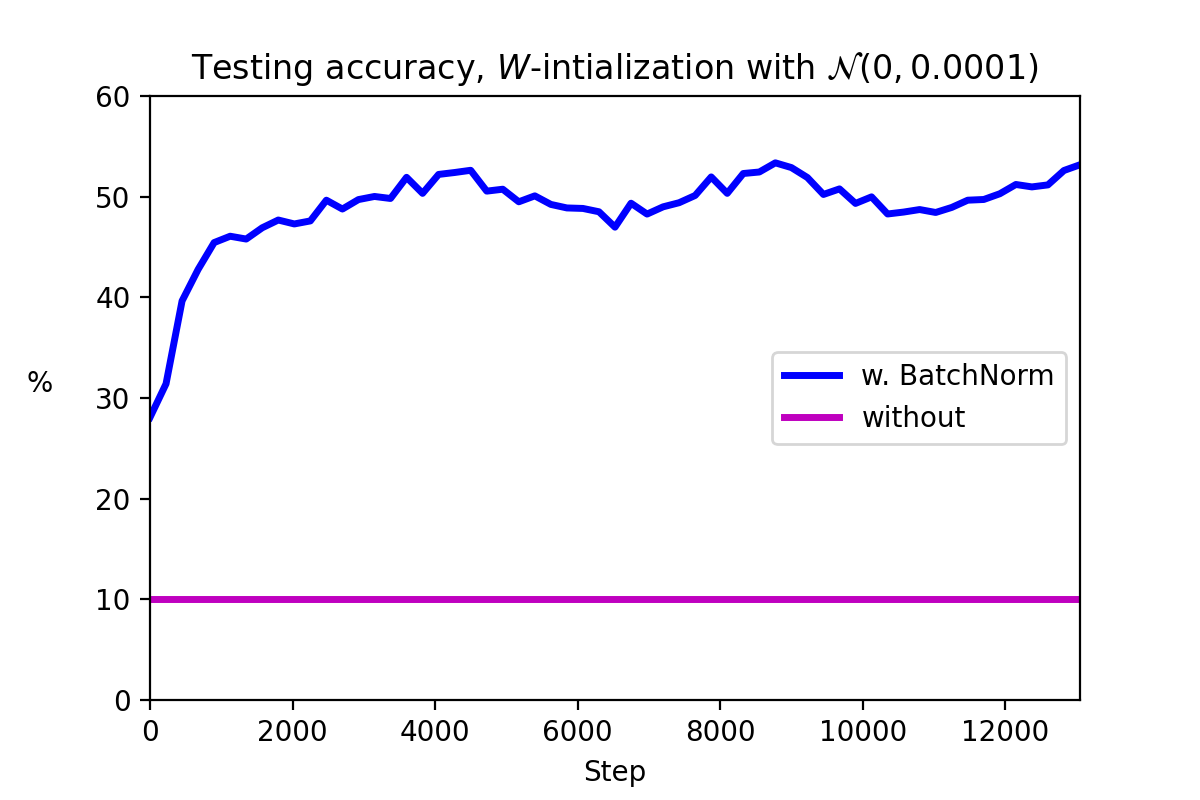
\includegraphics[width=7cm]{../plots/acc_comp_sigma3.png}
		\caption{Loss and accuracy for $3$-layer network with and without \texttt{batch normalization}, using $\lambda=0.005$, and a cyclical learning rate with $\eta_{min} = 10^{-5}$ and $\eta_{max} = 10^{-1}$, as well as random normal initialization for $\bm{W}$, with $\sigma\in\{10^{-1}, 10^{-3}, 10^{-4}\}$.}
	\end{figure}

\end{document}